Data in Mongodb has flexible schema where collections do not enforce document structure rather requirements of our application. There are two principle that allow application to represent documents and their relationship: \textit{reference} and \textit{embedded documents}. 

\todo{ need to change following image according to xmark data}
\begin{figure}
	\centering
	\subfigure[Reference document]{
		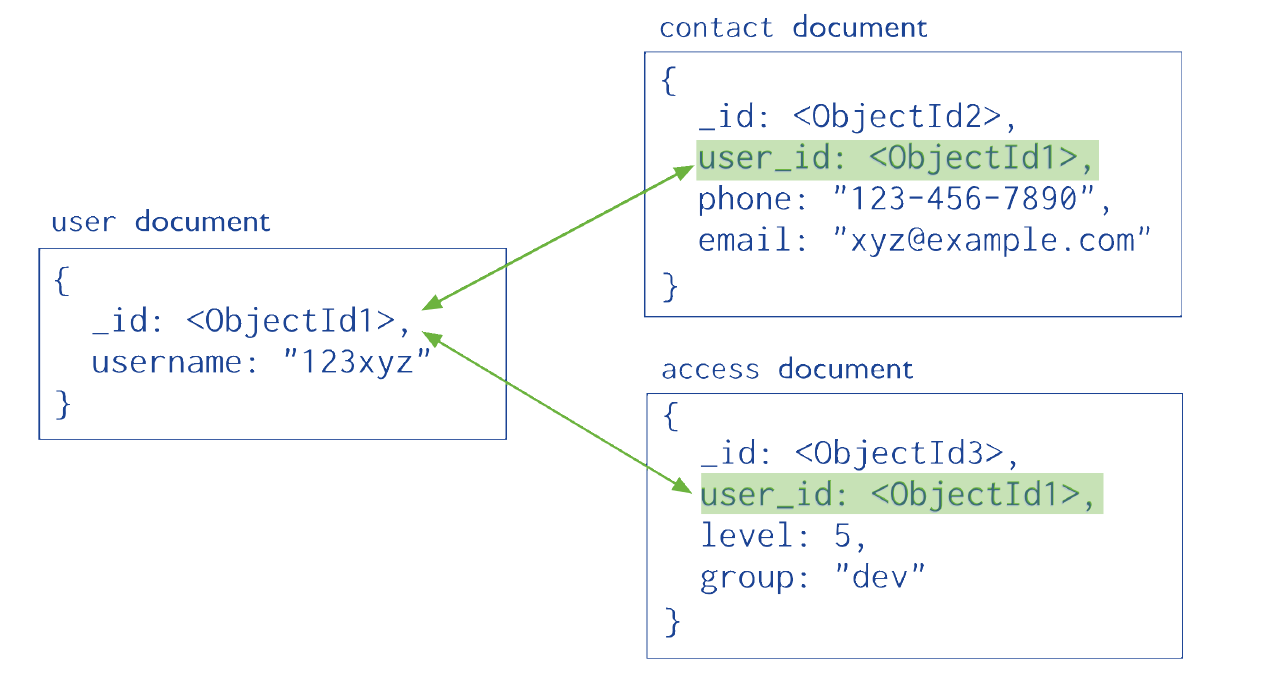
\includegraphics[width=0.44\textwidth]{img/mongodb-reference}
		%\caption{R-tree structure}
		\label{fig:mongodb-ref-doc}
	}
	\centering
	\subfigure[Embedded document]{
		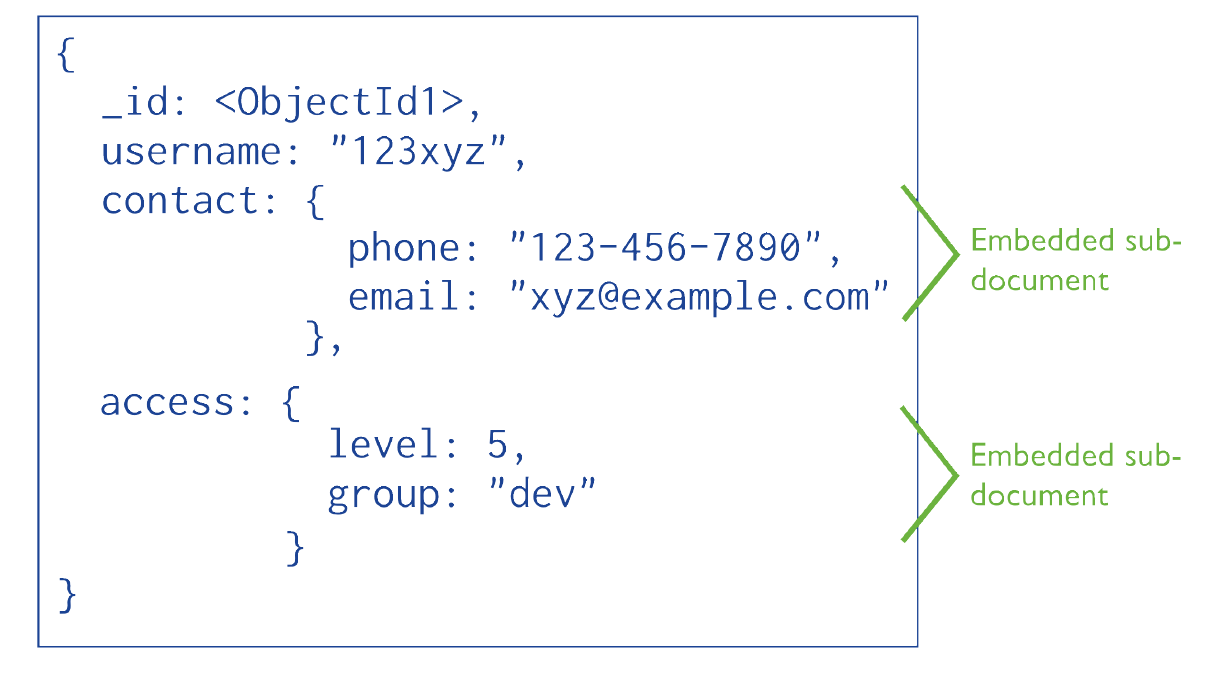
\includegraphics[width=0.44\textwidth]{img/mongodb-embedded}
		%\caption{R-tree}
		\label{fig:mongodb-emb-doc}
	}
	\caption{Mongodb document structure}
	\label{fig:mongodb-doc}
	 
\end{figure}

\paragraph{Reference}
		Reference store the relationships between data by including links and references from one document to another as in  Figure~\ref{fig:mongodb-ref-doc}. The application can resolve these reference to access the related data\todo{Mongodb data model pg4}
\paragraph{Embedded}
	Embedded documents captures relationships between the data by storing related data in a single document structure. The documents in this method are structured as sub-documents\todo{...??} in the in the form of Array or Object. 
